\documentclass[10pt,a4paper]{article}
\usepackage{amssymb,amsmath,graphicx}
\usepackage[utf8]{inputenc}
%\usepackage{newtxtext, newtxmath}
\usepackage[german]{babel}
\usepackage{caption}
\usepackage{subcaption}
\usepackage{verbatim}
\usepackage{eqnarray}
\usepackage{booktabs}

\def\permille{\ensuremath{{}^\text{o}\mkern-5mu/\mkern-3mu_\text{oo}}}

\setlength{\parindent}{0pt}

\begin{document}

\centerline{\large Sheet 7}\vspace{0.5em}
\centerline{\large von Benedikt Hemmer und Tobias Schmitt}\vspace{2em}

\section*{7a}

Wir berechnen die standartisierten $\delta$-Werte mit der folgenden Gleichung: 

\begin{align*}
\delta^{16} O_{VSMOW} &= \delta^{18} O_{WS} - 1.336 \, \permille \\
\delta^{2} H_{VSMOW} &= \delta^{2} H_{WS} - 88 \, \permille 
\end{align*} 	

Die resultierenden Werte sind in Tabelle \ref{tab:standardised} aufgeführt.

\begin{center}
\begin{tabular}{ccc}
height [m] & $\delta^{18} O_{VSMOW}$ [\permille] & $\delta^{2} H_{VSMOW}$ [\permille] \\ \midrule
\input{standardised.txt}

\end{tabular}
\captionof{table}{Standardisierte Daten gemessen im Willersinnweiher}
\label{tab:standardised}
\end{center}

\clearpage

\section*{7b}

In Abbildung \ref{fig:value_data} sehen wir, dass die gemessenen Werte von der LMWL abweichen. Sie liegen auf einer Gerade mit geringerer Steigung.
Dies ist darauf zurück zu führen, dass das Seewasser verdunstet und dabei Fraktionierung auftritt. Allerdings findet die Verdunstung nicht im vollständigen Gleichgewicht statt, was zu einer anderen Steigung führt. Dies ist z.B. auch aus dem Mittelmeer bekannt. Das zurückbleibende Wasser hat somit ebenfalls eine geändertes Isotopen-Verhältnis. Dies wird dadurch gestützt, dass das "schwerere" Wasser an der Oberfläche gemessen wurde und diese Datenpunkte dort gleichzeitig am weitesten von der LMWL entfernt liegen. 

\begin{figure}[ht]
\centering
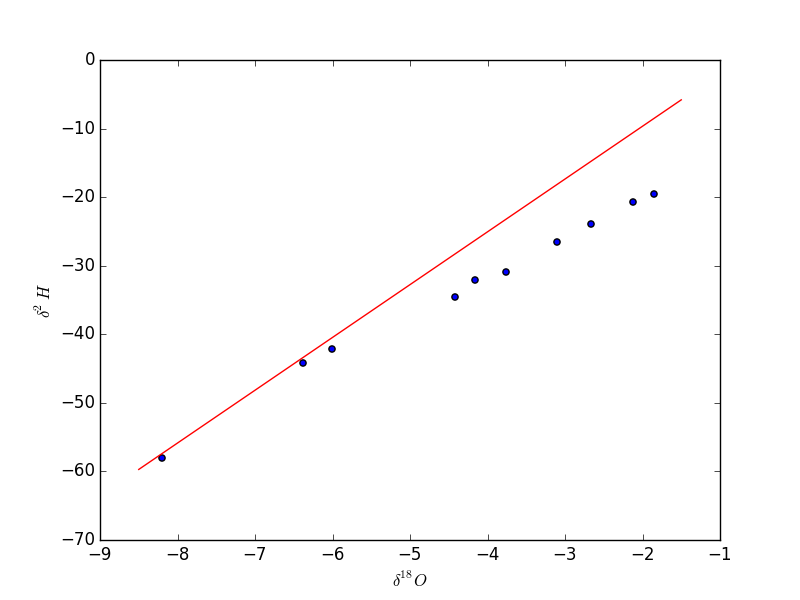
\includegraphics[width=1\linewidth]{plot_data_LMWL.png}
\caption{Plot der Messdaten vom Willersinnweiher mit LMWL}
\label{fig:value_data}
\end{figure}

\clearpage
\section*{7c}

Die folgenden Aussagen beziehen sich lediglich auf die $\delta^{18} O$ Werte, da die Werte für Wasserstoff teilweise nicht bekannt sind. \\ 
Zunächst ist festzustellen, dass das Wasser im Süden (Brunnen C) am leichtesten ist und sehr nah beim lokalen Grundwasser liegt. Dies ist im Norden (Brunnen A und B) nicht der Fall, dies ist deutlich schwerer.
Unter der Annahme, dass die Brunnen alle in einer ähnlichen Distanz zum See gebohrt wurden und das Grundwasser gleichmäßig geleitet wird, würden wir bei einfacher Diffusion ähnliche Werte bei allen drei Brunnen erwarten. Die Tatsache, dass bei C etwa Grundwasser vorliegt, lässt vermuten, dass die Interaktion mit dem See größtenteils durch Advektion stattfindet ($\rightarrow$ Grundwasserfluss durch den See).\\
Dies würde allerdings weder erklären, wieso erstens die Werte für Brunnen A und B verschieden sind, noch weshalb zweitens das Wasser am Boden des Sees auf der LMWL liegt aber schwerer als das Grundwasser ist. Es ist anzunehmen dass das Zufluss-Wasser des Sees auf der LMWL liegt (Niederschlag). Da das erneuernde Wasser auf der LMWL liegen muss, muss dieses den Schnittpunkt der LMWL mit der "Verdunstungslinie" markieren. Dies widerspricht der Annahme, dass der See sich aus dem Grundwasser speist (siehe fig. \ref{fig:value_data}).
Eine mögliche Erklärung wäre, dass nur geringer Austausch mit der Region um Brunnen C besteht und der See sich aus z.B. lokalem Regenwasser speist.\\
Die Unterscheide in den Brunnen A und B lassen sich dadurch erklären, dass die Flüsse vom See ins Grundwasser bei unterschiedlichen Höhen stattfinden. Die Unterschiede sind dann direkt auf die Schichtung des Sees zurückzuführen. Alternativ sind sie u.A. durch verschiedenen Brunnentiefen in Kombination mit geringen vertikalen Leitwerten (sodass sich die Schichtung im Grundwasser fortsetzt) zu erklären oder unterschiedlichen Abständen zum See, sowie unterschiedlichen horizontalen Leitwerten.

\newpage

\section*{Python script used for exercise}
\verbatiminput{uebung7.py}

\end{document}
